\let\negmedspace\undefined
\let\negthickspace\undefined
\documentclass[journal]{IEEEtran}
\usepackage[a5paper, margin=10mm, onecolumn]{geometry}
\usepackage{tfrupee}

\setlength{\headheight}{1cm}
\setlength{\headsep}{0mm}

\usepackage{gvv-book}
\usepackage{gvv}
\usepackage{cite}
\usepackage{amsmath,amssymb,amsfonts,amsthm}
\usepackage{algorithmic}
\usepackage{graphicx}
\usepackage{textcomp}
\usepackage{xcolor}
\usepackage{txfonts}
\usepackage{listings}
\usepackage{enumitem}
\usepackage{mathtools}
\usepackage{gensymb}
\usepackage{comment}
\usepackage[breaklinks=true]{hyperref}
\usepackage{tkz-euclide}
\usepackage{listings}
\def\inputGnumericTable{}
\usepackage[latin1]{inputenc}
\usepackage{color}
\usepackage{array}
\usepackage{longtable}
\usepackage{calc}
\usepackage{multirow}
\usepackage{hhline}
\usepackage{ifthen}
\usepackage{lscape}

\begin{document}

\bibliographystyle{IEEEtran}
\vspace{3cm}

\title{4.9.5}
\author{EE25BTECH11003 - Adharvan Kshathriya Bommagani}
{\newpage\maketitle}

\renewcommand{\thefigure}{\theenumi}
\renewcommand{\thetable}{\theenumi}
\setlength{\intextsep}{10pt}

\textbf{Question}:\\
Equations of the lines through the point (3,2) and making an angle of 40\degree with the line $x - 2y = 3$ are.

\bigskip

\textbf{Solution}:\\



First, we express the given point and line using column vectors.\\
The line passes through the point $(3, 2)$. We can represent this with a position vector $\vec{h}$:
$$ \vec{h} = \myvec{3 \\ 2} $$
The given line is $x - 2y = 3$. From the formula $\vec{n}^\top \vec{x} = c$, we can identify the \textbf{normal vector} to this line, which we'll call $\vec{n_1}$:
$$ \vec{n_1} = \myvec{1 \\ -2} $$
The \textbf{direction vector} of a line, $\vec{m_1}$, is orthogonal to its normal vector, meaning $\vec{m_1}^\top \vec{n_1} = 0$. A simple choice is:
$$ \vec{m_1} = \myvec{2 \\ 1} $$


We need to find the direction vectors, $\vec{m_2}$ and $\vec{m_3}$, for the new lines by rotating the known direction vector $\vec{m_1}$ by both $+40\degree$ and $-40\degree$. The rotation matrix $R(\theta)$ is:
$$ R(\theta) = \begin{pmatrix} \cos\theta & -\sin\theta \\ \sin\theta & \cos\theta \end{pmatrix} $$
\textbf{For the first line (rotation by +40\degree):}
\begin{align*}
\vec{m_2} = R(40\degree) \vec{m_1} &= \begin{pmatrix} \cos(40\degree) & -\sin(40\degree) \\ \sin(40\degree) & \cos(40\degree) \end{pmatrix} \myvec{2 \\ 1} \\
&= \myvec{2\cos(40\degree) - \sin(40\degree) \\ 2\sin(40\degree) + \cos(40\degree)}
\end{align*}
\textbf{For the second line (rotation by -40\degree):}
\begin{align*}
\vec{m_3} = R(-40\degree) \vec{m_1} &= \begin{pmatrix} \cos(40\degree) & \sin(40\degree) \\ -\sin(40\degree) & \cos(40\degree) \end{pmatrix} \myvec{2 \\ 1} \\
&= \myvec{2\cos(40\degree) + \sin(40\degree) \\ -2\sin(40\degree) + \cos(40\degree)}
\end{align*}


We use the vector equation of a line, $\vec{x} = \vec{h} + \kappa \vec{m}$, and convert it to Cartesian form.






The normal form is $\vec{n}^\top \vec{x} = c$, where $c = \vec{n}^\top \vec{h}$. A normal vector $\vec{n}$ can be obtained from a direction vector $\vec{m} = \myvec{u \\ v}$ as $\vec{n} = \myvec{-v \\ u}$.\\

\textbf{First Line in Normal Form:}\\
The normal vector $\vec{n_2}$ from $\vec{m_2}$ is:
$$ \vec{n_2} = \myvec{-(2\sin(40\degree) + \cos(40\degree)) \\ 2\cos(40\degree) - \sin(40\degree)} $$
The constant $c_2 = \vec{n_2}^\top \vec{h}$ is:
\begin{align*}
c_2 &= [-(2\sin(40\degree) + \cos(40\degree)), \quad 2\cos(40\degree) - \sin(40\degree)] \myvec{3 \\ 2} \\
&= -3(2\sin(40\degree) + \cos(40\degree)) + 2(2\cos(40\degree) - \sin(40\degree)) \\
&= \cos(40\degree) - 8\sin(40\degree)
\end{align*}
The equation is:
$$ \myvec{-(2\sin(40\degree) + \cos(40\degree)) \\ 2\cos(40\degree) - \sin(40\degree)}^\top \myvec{x \\ y} = \cos(40\degree) - 8\sin(40\degree) $$\\

\textbf{Second Line in Normal Form:}\\
The normal vector $\vec{n_3}$ from $\vec{m_3}$ is:
$$ \vec{n_3} = \myvec{-(-2\sin(40\degree) + \cos(40\degree)) \\ 2\cos(40\degree) + \sin(40\degree)} = \myvec{2\sin(40\degree) - \cos(40\degree) \\ 2\cos(40\degree) + \sin(40\degree)} $$
The constant $c_3 = \vec{n_3}^\top \vec{h}$ is:
\begin{align*}
c_3 &= [2\sin(40\degree) - \cos(40\degree), \quad 2\cos(40\degree) + \sin(40\degree)] \myvec{3 \\ 2} \\
&= 3(2\sin(40\degree) - \cos(40\degree)) + 2(2\cos(40\degree) + \sin(40\degree)) \\
&= \cos(40\degree) + 8\sin(40\degree)
\end{align*}
The equation is:
$$ \myvec{2\sin(40\degree) - \cos(40\degree) \\ 2\cos(40\degree) + \sin(40\degree)}^\top \myvec{x \\ y} = \cos(40\degree) + 8\sin(40\degree) $$

\newpage
\textbf{Plot of the Lines:}
\begin{figure}[H]
    \centering
    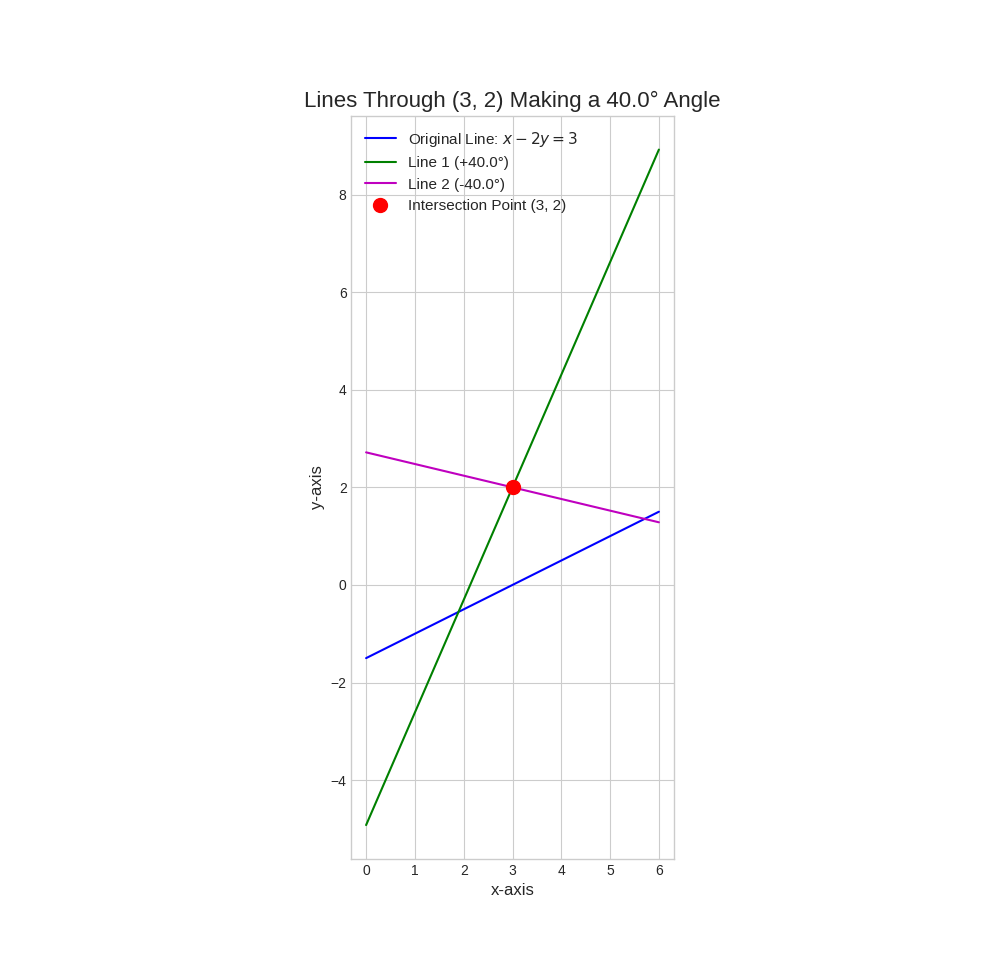
\includegraphics[width=1.1\columnwidth]{figs/fig1.png}
    \caption{Figure for 4.9.5}
    \label{}
\end{figure}



\end{document}